The following chapter is included to show that the developed hybrid diffusion solver can be applied to real life problems with only minor modifications.

\section{Physical scope}


\emph{\textcolor{red}{Her bør det stå noe om hva vi holder på med og hvor det kommer fra, samt hvorfor det er interessant og hva vi faktisk kommer til å måle (diffusjonstid for walkers gjennom spine neck).}}

PKC$\gamma$ is associated with memory storage and will diffuse out of the cell body (soma) of a neuron through a dendrite into a dendritic spine to reinforce the absorption of neurotransmitters. 
This application is aimed at modeling PKC$\gamma$ diffusion in a dendrite and into spines. 
Because of symmetry the dendrite will be modeled as 1D continuous diffusion while the diffusion in spines will be modeled as a random walk. 
Effectively we will investigate the diffusion time for random walkers through spine necks which are very narrow ($\leq0.5\mu$m). 
The results will be compared to results by Craske et.al \cite{craske2005spines}.

\section{Implementation}

There is a difference between the approach of the developed hybrid solver and the dendrite - spine system with respect to geometry which is best summarized in figure \ref{application:geometry_difference}.

\begin{figure}[H]
 \centering
 \begin{subfigure}{0.48\textwidth}
  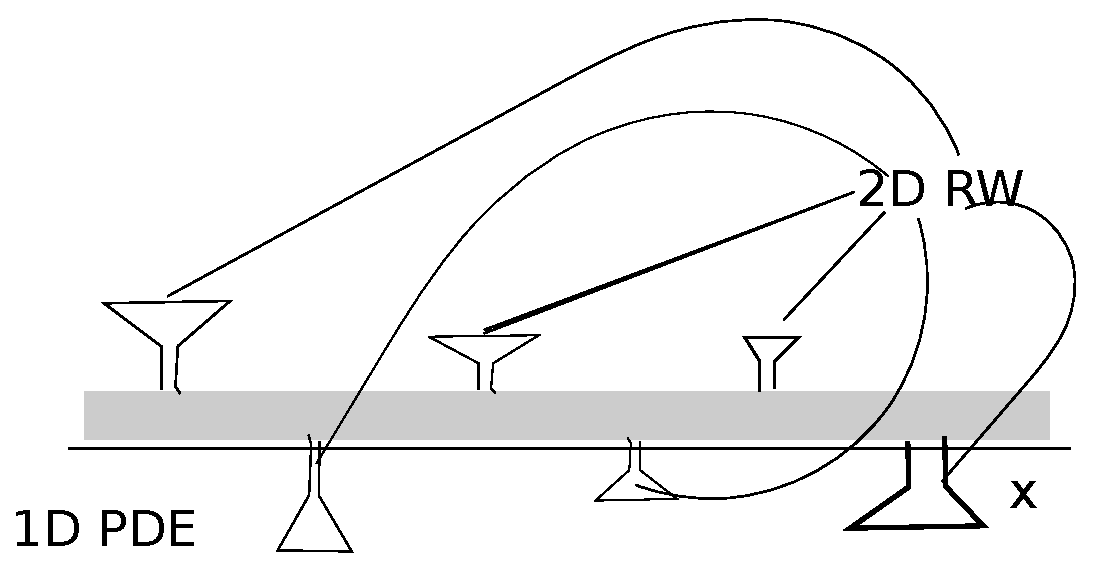
\includegraphics[width=\textwidth]{Figures/dendrite_spine_model.eps}
  \caption{}
 \end{subfigure}
 \begin{subfigure}{0.48\textwidth}
  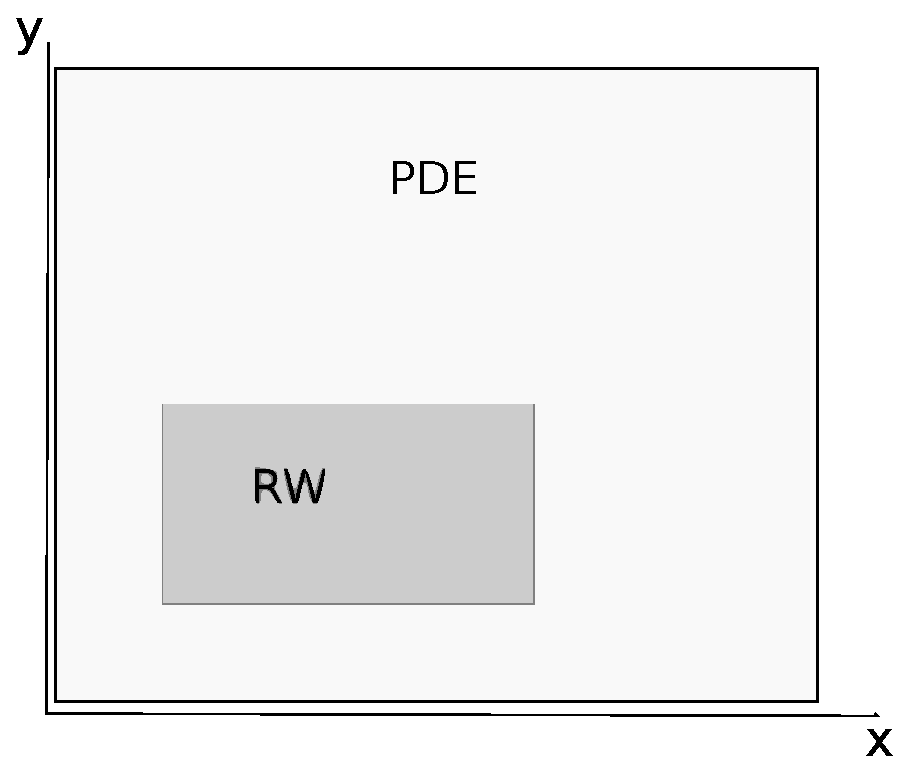
\includegraphics[width=\textwidth]{Figures/hybrid_model_principle.eps}
  \caption{}
 \end{subfigure}
 \caption[Difference between hybrid diffusion solver and dendrite - spine diffusion model]{The geometric difference between the original hybrid diffusion solver (b) and the problem of PKC$\gamma$ diffusing into dendritic spines (a). }
 \label{application:geometry_difference}
\end{figure}

The hybrid diffusion solver has been slightly modified in order to recreate the new geometry. 
Mathematically the largest difference is that the random walkers are left alone, meaning that the diffusion equation is not solved in the spines. 
There are also some differences in the coupling; at each PDE time step there is a probability for an enzyme to diffuse into a spine if the concentration at the beginning of the spine neck is large enough. This probability decreases with the number of enzymes which have already diffused into the spine. 
The width of a spine neck is determined by the number of PDE mesh points it connects to, all other length parameters are determined randomly but required to fit with measurements from Arrelano et.al \cite{arellano2007ultrastructure}. 

\clearpage

\section{Parameters}

The new problem requires the introduction of some additional parameters as well as a reformulation of limiting factors for some known parameters, all of which are described in the following table.
 
 \begin{table}[H]
\centering
\begin{tabular}{|p{0.13\textwidth}|p{0.21\textwidth}|p{0.18\textwidth}|p{0.37\textwidth}|}
\hline
\textbf{Parameter} & \textbf{Explanation} &\textbf{Expression/ typical value}& \textbf{Origin} \\
\hline
$\Delta t$ & time-step & $\Delta x^2$ & stability criterion FE scheme \\
\hline
$\Delta x$ & spatial resolution & $\frac{1}{2}$min(spine neck diameter) & estimated \\
\hline
$Hc$ & conversion factor & 5-24 & estimated by calculations of concentration levels taken from \cite{light1996protein} and spine/dendrite volume ratios. See later for discussion. \\
\hline
$u(t=0)$ & initial condition value & 5$\frac{\text{nMol}}{\text{L}}$ & estimated from values found in \cite{light1996protein}\\
\hline
$p_{ds}$ & probability to diffuse into a spine & $0.1\cdot\Delta x\cdot\Delta t$& estimated. An important ability of this parameter should be that wide necked spines have larger probability and that a certain flux is maintained (on average), meaning that the flux should be independent of $\Delta t$ \\
\hline
$p_{ab}$ & probability for PKC$\gamma$ to be absorbed, and removed from simulation, per time-step taken in spine head & 100\% & estimated\\
\hline
\end{tabular}
\caption[Important parameters]{Parameters which play an important role in the simulation of PKC$\gamma$ diffusion into dendritic spines with explanations, expressions/typical values and an indication as to where the value/expression has its origin.}
\label{table:parameters}
\end{table}
